% LTex: language=pl

\section{Konteneryzacja i rozwiązania alternatywne}
\subsection{Wirtualizacja}
Pojęcie wirtualizacji zaczęło pojawiać się w użyciu już w latach siedemdziesiątych XX wieku. W 1974 opublikowany został artykuł autorstwa Geralda J. Popka i Roberta P. Goldberga, którego autorzy wprowadzili sformalizowaną definicję wirtualizacji. Główne założenia proponowanej definicji opierały się na twierdzeniu o zachowaniu relacji równoważności pomiędzy pojedynczymi instrukcjami i sekwencjami instrukcji wykonywanymi na maszynie fizycznej i maszynie wirtualnej \cite{virtualization}.

\begin{lemat}
	Niech $i$ oznacza dowolną instrukcję, $S$ oznacza stan maszyny fizycznej, natomiast $S'$ stan maszyny wirtualnej, w taki sposób, że $S' = f(S)$. Wykonanie instrukcji na obu maszynach wiąże się z identyczną interpretacją takiej instrukcji w obu środowiskach, tak że $i(S) = i(S')$.
\end{lemat}

\begin{lemat}
	Ponieważ wszystkie pojedyncze instrukcje $i$ interpretowane są w ten sam sposób na maszynie fizycznej o stanie $S$ i maszynie wirtualnej o stanie $S'$, wszystkie skończone zbiory uporządkowane instrukcji $t = (i_1, i_2, \ldots, i_n)$ również interpretowane są w ten sam sposób dla obu środowisk, tak że $f(t(S)) = f(t(S'))$.
\end{lemat}

\noindent Oprócz formalnych dowodów dotyczących zachowania maszyny i właściwości, jakie powinna wykazywać, artykuł ten wprowadził pojęcie "monitora maszyny wirtualnej" - programu zarządzającego zachowaniem i zasobami wirtualizowanej maszyny i wskazał również główne moduły składające się na taki program. Na przestrzeni lat pojęcie to przekształciło się w "nadzorcę" \textit{(hypervisor)}, wraz z podziałem na 2 główne typy programu-nadzorcy -- nadzorca typu pierwszego \textit{(type 1 hypervisor)} i nadzorca typu drugiego \textit{(type 2 hypervisor)}.

\noindent O wiele młodszą technologią jest z kolei konteneryzacja, która, mimo podobieństwa do wirtualizacji, nie spełnia wszystkich wymogów formalnych prezentowanych powyżej, w szczególności tych, dotyczących zachowania relacji równoważności pomiędzy pojedynczymi instrukcjami procesora i powiązania wyłącznie z architekturą fizyczną maszyny. Mimo tego jest ona szeroko wykorzystywana w rozwiązaniach o szerokim spektrum skali -- od projektów hobbystycznych do rozwiązań klasy przemysłowej.

\subsection{Kontenery a maszyny wirtualne}
W celu przedstawienia głównych różnic pomiędzy wirtualizacją i konteneryzacją należy przeanalizować architekturę rozwiązań implementujących te technologie -- silnik konteneryzacji, nadzorcę typu pierwszego \textit{(type 1 hypervisor)} i nadzorcę typu drugiego \textit{(type 2 hypervisor)} (rysunek \ref{diagramWirtualizacja}).

\begin{figure}[!h]
	\begin{center}
		\resizebox{0.7\textwidth}{!} {
			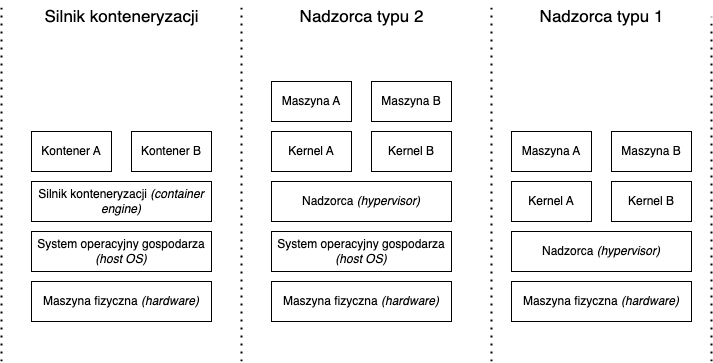
\includegraphics{img/4/wirtualizacja.png}
		}
		\caption[Porównanie silnika konteneryzacji i programów-nadzorców]{Schemat przedstawiający i porównujący architekturę silnika konteneryzacji i programów-nadzorców maszyn wirtualnych. Źródło własne.}
		\label{diagramWirtualizacja}
	\end{center}
\end{figure}

\subsubsection{Nadzorca typu pierwszego \textit{(type 1 hypervisor)}}
Programy nadzorcy typu pierwszego najczęściej wykorzystywane są w rozwiązaniach przemysłowych, wymagających zaawansowanych rozwiązań z zakresu monitorowania nadzorowanych maszyn wirtualnych i wydajności przetwarzania. Do najpopularniejszych ogólnodostępnych programów zaliczających się do tej rodziny należą, między innymi, Proxmox, xcp-ng i KVM. Nadzorca typu pierwszego pełni rolę systemu operacyjnego zainstalowanego na maszynie fizycznej i posiada bezpośrednią kontrolę nad jej zasobami sprzętowymi. Dzięki temu wirtualizacja realizowana przy pomocy oprogramowania tego typu charakteryzuje się blisko natywną wydajnością wirtualizowanych maszyn. Każda maszyna wirtualna stanowi w pełni oddzielną maszynę logiczną, z wydzielonym jądrem systemu operacyjnego i dedykowaną ilością zasobów fizycznych, takich jak pamięć operacyjna czy rdzenie lub wątki procesora. Ponadto, z racji ich powszechnego wykorzystania w rozwiązaniach klasy przemysłowej, bardzo często programy-nadzorcy typu pierwszego posiadają wbudowane funkcjonalności zarządzania systemami (klastrami) składającymi się z wielu maszyn fizycznych podobne do rozwiązań obecnych w systemach orkiestracji kontenerów, takich jak Kubernetes.

\subsubsection{Nadzorca typu drugiego \textit{(type 2 hypervisor)}}
Nadzorca typu drugiego to najbardziej rozpowszechniony program oferujący pełną wirtualizcję. Reprezentantami tej rodziny programów-nadzorców maszyn wirtualnych są programy Oracle VirtualBox, Parallels i VMware. Nadzorca typu drugiego to program uruchamiany na dowolnej maszynie z uprzednio zainstalowanym systemem operacyjnym, co czyni go najbardziej przyjaznym rozwiązaniem do celów konsumenckich lub prototypowania. Mimo instalacji na istniejącym systemie nadzorca typu drugiego oferuje te same funkcjonalności związane z wirtualizacją co nadzorca typu pierwszego, alokując dedykowane zasoby dla poszczególnych maszyn wirtualnych, którymi zarządza, w tym osobny kernel (jądro) systemu dla każdej maszyny logicznej. Wygoda użytkowania niesie za sobą jednak koszty związane z wydajnością maszyn, ponieważ system operacyjny, na którym uruchomiony jest program-nadzorca wnosi znaczące opóźnienia związane z komunikacją systemu w maszynie wirtualnej z zasobami sprzętowymi kontrolowanymi przez system operacyjny gospodarza. Ponadto, funkcjonalności takie jak zarządzanie systemami składającymi się z wielu maszyn fizycznych nie są wbudowane w programy zaliczające się do tej rodziny, zamiast tego nacisk kładziony jest na łatwość użytkowania aplikacji przez użytkownika końcowego.

\subsubsection{Silnik konteneryzacji}
Konteneryzacja to technologia, pozwalająca na uzyskanie większości funkcjonalności wirtualizacji wykorzystując stosunkowe małe maszyny logiczne nazywane "kontenerami". Główna różnica pomiędzy wirtualizacją i konteneryzacją polega na wykorzystaniu systemu operacyjnego gospodarza. O ile w przypadku wirtualizacji, z wykorzystaniem nadzorcy typu pierwszego i drugiego, każda maszyna wirtualna posiada swój własny kernel (jądro) systemu operacyjnego, w przypadku konteneryzacji system operacyjny, w szczególności jego jądro, jest współdzielone między wszystkie kontenery. Skutkuje to zmniejszeniem rozmiaru kontenerów, które nie muszą zawierać w sobie obrazu całego systemu i szybszym czasem uruchamiania, które są często głównymi czynnikami przemawiającymi za zastosowaniem kontenerów nad maszynami wirtualnymi. Jednakże, z racji ścisłego powiązania z systemem gospodarza, na którym działa kontener, lemat dotyczący zachowania relacji równoważności instrukcji dotyczący maszyny wirtualnej Popka i Goldberga \cite{virtualization} nie jest zachowany dla każdego kontenera uruchomionego na tej samej architekturze. Przykładowo, kontener oparty na systemie Linux może zostać uruchomiony na maszynach gospodarza o różnych wersjach kernela (jądra) systemu, rezultatem czego może być różna interpretacja wywołań systemowych dla identycznych wywołań w każdym z tych kontenerów. Dlatego, w świetle tego artykułu, konteneryzacja nie jest stricte rodzajem wirtualizacji. Z praktycznego punktu widzenia, oznacza to niemożność wykorzystania kontenerów opartych na pewnym systemie operacyjnym $O_a$ na maszynie o systemie operacyjnym $O_b$, gdzie kernele (jądra) systemów $O_a$ i $O_b$ są ze sobą niekompatybilne -- przykładem takiej sytuacji jest próba uruchomienia kontenera korzystającego z systemu Microsoft Windows ($O_a$) na maszynie opartej na systemie Linux ($O_b$).

\subsection{Wirtualizacja a platforma serwerowa dla systemu STOS}
Z racji wystąpienia komplikacji, o których była mowa w poprzednim podrozdziale, w ramach poszukiwania rozwiązania alternatywnego dla konteneryzacji, naturalnym wyborem była analiza wirtualizacji jako technologii stanowiącej podstawę wdrożenia systemu. Pierwszą decyzją, którą należało podjąć, był wybór typu nadzorcy \textit{(hypervisor)} i konkretnej implementacji tego rozwiązania. W świetle doświadczeń z systemami orkiestracji kontenerów naturalnym wyborem był system oparty na nadzorcy typu pierwszego \textit{(type 1 hypervisor)}; wiele z implementacji tego właśnie typu nadzorcy oferuje funkcjonalności z zakresu zarządzania wieloma maszynami fizycznymi, co było jednym z wymagań dla wdrożonego systemu. Dwiema implementacjami takiego systemu, których zastosowanie było rozważane, były Proxmox i xcp-ng \cite{proxmox, xcp}. Oba z tych rozwiązań oferują bardzo podobne rozwiązania, lecz ostatecznie wybrano xcp-ng jako system nadzorcy, na podstawie którego realizowana jest wirtualizacja serwisów w ramach platformy serwerowej dla systemu STOS.
